%% 06_model2_bank_stress.tex
%% Section 6: Model 2 -- Banking Sector Stress Test

\section{Model 2: Banking Sector Stress Test}
\label{sec:model2}

The second model traces how coal stranding propagates to the banking sector through credit exposures. We construct a bipartite bank-coal exposure network from granular loan data, classify coal companies by default status under each scenario, and estimate the resulting credit losses and capital adequacy impacts for each bank.

\subsection{Bank-Coal Exposure Network}
\label{subsec:bipartite_network}

The foundation of our stress test is a bipartite network linking banks to coal companies through identified credit relationships. We construct this network from annual report disclosures of 38 listed banks, which report their largest borrower exposures by company name, loan amount, currency, and sector classification. For coal companies, we identify direct credit facilities, including term loans, revolving credit, project finance, and trade finance, extended by each bank to each coal company in our sample.

Let $W_{b,c}$ denote the exposure of bank $b$ to coal company $c$, measured in USD millions after currency conversion. The exposure matrix $\mathbf{W}$ has dimensions $B \times C$, where $B = 13$ banks with identified coal exposures (of the 38 in our sample) and $C = 26$ coal companies receiving bank credit. The total identified exposure is \$6.1 billion, of which \$3.3 billion (53.8\%) is attributed to specific bank-company pairs. The remaining \$2.8 billion is classified under aggregate categories (foreign banks, syndicated loans, and other domestic banks) that cannot be traced to individual institutions in our sample.

Figure~\ref{fig:network} visualises the bipartite network. The network exhibits substantial concentration: four domestic systemically important banks (D-SIBs), namely Bank Mandiri (BMRI), Bank Negara Indonesia (BBNI), Bank Central Asia (BBCA), and Bank Rakyat Indonesia (BBRI), account for 79\% of identified bank-level coal exposure. BMRI alone holds \$1.2 billion in direct coal lending, representing the largest single-bank exposure in the network. On the coal company side, the top five borrowers absorb over 60\% of total bank credit to the sector.

\begin{figure}[htbp]
\centering
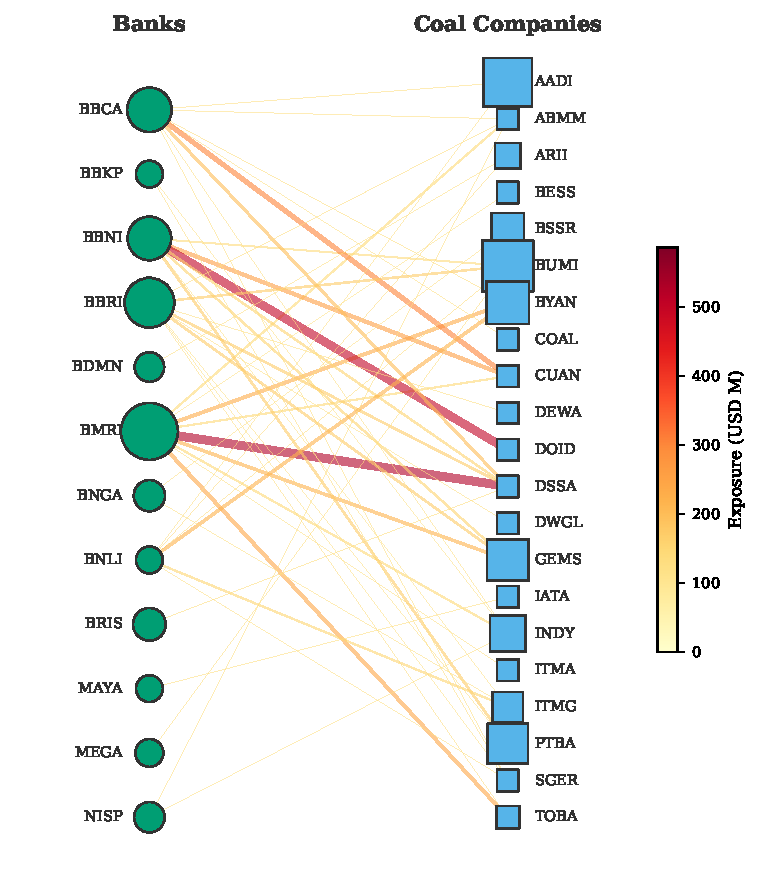
\includegraphics[width=\textwidth]{figures/fig_05.pdf}
\caption{Bipartite bank-coal exposure network. Left nodes represent banks (circle size proportional to total assets); right nodes represent coal companies (square size proportional to annual production). Edge width is proportional to loan exposure in USD millions. The four D-SIBs are highlighted in darker shading.}
\label{fig:network}
\end{figure}

In addition to direct identified exposures, banks hold mining sector loans that may include coal-related lending not individually identified in the bipartite network. We capture these ``indirect'' exposures using the mining loan data from bank financial statements. For bank $b$, the indirect coal exposure is estimated as:
\begin{equation}
\label{eq:indirect}
E_b^{indirect} = M_b - \sum_{c} W_{b,c}
\end{equation}
where $M_b$ is the bank's total mining sector loans (from sectoral loan disclosures) and $\sum_c W_{b,c}$ is its total identified coal exposure. This residual captures lending to unlisted coal companies, coal service providers, and other mining sub-sectors that may be indirectly affected by coal stranding.

\subsection{Credit Loss Model}
\label{subsec:credit_loss}

We model credit losses in two stages: first, we classify each coal company's credit status under each scenario using Model 1 outputs; second, we compute the expected loss for each bank-coal pair.

\subsubsection{Coal Company Default Classification}

Each coal company $c$ is assigned a credit status $S_c^s \in \{\text{Default}, \text{Distressed}, \text{Performing}\}$ under scenario $s$ based on its NPV and equity position:

\begin{equation}
\label{eq:default}
S_c^s = \begin{cases}
\text{Default} & \text{if } NPV_c^s < 0 \\
\text{Distressed} & \text{if } NPV_c^s \geq 0 \text{ and } SV_c^s > 0.50 \cdot E_c \\
\text{Performing} & \text{otherwise}
\end{cases}
\end{equation}
where $E_c$ is the firm's total equity. The rationale is as follows: a negative NPV indicates that the firm's coal operations are value-destroying, implying eventual inability to service debt (default); a positive NPV but stranded value exceeding 50\% of equity indicates material financial stress that elevates credit risk without immediate default; otherwise, the firm remains performing.

We acknowledge that a negative NPV does not mechanically imply default. In the Merton (1974) structural credit risk framework, default occurs only when asset value falls below the default boundary (typically total liabilities), and firms with negative NPV coal operations may still service debt from cash reserves, non-coal revenue streams, or new equity issuance. Several companies in our sample, notably BYAN and AADI, maintain substantial cash positions that could sustain operations for several years even under negative-NPV coal operations. Our classification therefore represents a \textit{long-run} default assessment: firms whose core business is value-destroying will eventually face debt-servicing difficulties absent a strategic pivot. An alternative, more conservative specification would classify as defaulting only firms with $NPV_c^s < 0$ \textit{and} a cash-to-debt ratio below a threshold (e.g., 0.20). We leave this extension to future robustness analysis, noting that it would reduce the number of defaulting firms and lower aggregate credit losses.

Under the BAU scenario, 3 firms default, none are distressed, and 23 are performing; the remaining 8 lack the verified production data needed for NPV-based classification and are assigned a ``no data'' status. Under the 2\textdegree C scenario, 5 firms default and 21 have positive NPV (though many are distressed with stranded values exceeding 50\% of equity). Under the 1.5\textdegree C scenario, 10 firms default and 16 retain positive NPV. This deterioration reflects the severity of the climate-adjusted price paths, which push many producers below breakeven. The 8 firms without NPV data are excluded from the default classification, which means our credit loss estimates are conservative, capturing only losses from the 26 firms with verified cost and production data.

\subsubsection{Loss Given Default}

The loss given default (LGD) varies by credit status:

\begin{equation}
\label{eq:lgd}
LGD_c^s = \begin{cases}
\min\left(1, \frac{|NPV_c^s|}{D_c}\right) & \text{if } S_c^s = \text{Default} \\[6pt]
0.30 \times \frac{SV_c^s}{A_c} & \text{if } S_c^s = \text{Distressed} \\[6pt]
0 & \text{if } S_c^s = \text{Performing}
\end{cases}
\end{equation}
where $D_c$ is total debt and $A_c$ is total assets. For defaulting firms, the LGD is bounded by the ratio of the NPV shortfall to total debt, capped at 100\%. For distressed firms, we apply a 30\% multiplier scaled by the stranded value relative to assets. The 30\% multiplier is calibrated as follows: the Basel IRB Foundation approach assigns an LGD of 45\% for unsecured senior claims and 25\% for secured claims with recognised collateral. Since Indonesian coal loans are typically partially secured by mining concession rights and equipment (but not by liquid collateral), we adopt 30\% as an intermediate value. We note that no empirical LGD estimates specific to Indonesian coal sector defaults exist in the literature, which makes this a key source of model uncertainty; the robustness analysis in Section~\ref{subsec:robustness} tests sensitivity to LGD values ranging from 0.20 to 0.55. We also note that for highly distressed firms where stranded value far exceeds total assets, the computed LGD can exceed unity (e.g., GEMS, where the SV/A ratio reaches 3.95 under 1.5\textdegree C); in such cases we apply an explicit cap at 100\%. Performing firms incur no losses under our baseline specification, though we relax this assumption in robustness checks (Section~\ref{sec:discussion}).

\subsubsection{Bank-Level Credit Losses}

The total credit loss for bank $b$ under scenario $s$ comprises direct losses from identified exposures and indirect losses from residual mining portfolios:

\begin{equation}
\label{eq:bank_loss}
L_b^s = \underbrace{\sum_{c} W_{b,c} \cdot LGD_c^s}_{\text{Direct losses}} + \underbrace{E_b^{indirect} \cdot \Delta NPL^s \cdot LGD^{generic}}_{\text{Indirect losses}}
\end{equation}

The indirect loss term applies a scenario-dependent NPL increment $\Delta NPL^s$ (calibrated at 0.5 percentage points for BAU, 5 percentage points for 2\textdegree C, and 15 percentage points for 1.5\textdegree C) multiplied by a generic LGD of 45\%, consistent with Basel regulatory parameters for corporate exposures in emerging markets. The NPL shock calibration warrants discussion. The 15 percentage point increment under the 1.5\textdegree C scenario is applied to the \textit{residual} mining portfolio, which includes non-coal mining (nickel, tin, gold) that may not be directly affected by the coal transition. This is a conservative (loss-increasing) assumption. For context, the historical peak NPL ratio in the Indonesian mining sector was 7.7\% during the 2015--2016 commodity price downturn, when Newcastle coal prices fell to approximately \$48/tonne. Our 1.5\textdegree C NPL shock of 15 percentage points thus represents roughly twice the worst historical episode, reflecting the deeper and more sustained nature of the structural transition relative to a cyclical price downturn. The sensitivity of stress test results to alternative NPL shock specifications is discussed in Section~\ref{subsec:robustness}.

\subsection{Capital Adequacy Impact}
\label{subsec:capital_adequacy}

We assess the impact on each bank's capital adequacy ratio (CAR) by deducting credit losses from equity capital:

\begin{equation}
\label{eq:car_impact}
CAR_b^{post} = \frac{E_b - L_b^s}{RWA_b}
\end{equation}
where $E_b$ is pre-stress equity capital, $L_b^s$ is the total credit loss, and $RWA_b$ is risk-weighted assets. We hold RWA constant, which introduces two offsetting biases. On one hand, this understates the CAR impact because defaulted exposures should migrate to a 150\% risk weight under Basel standardised rules, increasing the denominator and further compressing the post-stress CAR. On the other hand, holding RWA constant overstates the impact to the extent that existing loan loss provisions (CKPN) would absorb losses before they reach equity, reducing the numerator deduction. The net direction of bias is unclear and likely bank-specific; we acknowledge this as a simplifying assumption. The CAR impact in percentage points is:
\begin{equation}
\label{eq:car_delta}
\Delta CAR_b^s = \frac{L_b^s}{RWA_b} \times 100
\end{equation}

We benchmark post-stress CARs against two regulatory thresholds: the OJK minimum CAR of 8\% (applicable to all banks) and the enhanced capital buffer for D-SIBs, which ranges from 10.5\% to 13\% depending on the bank's systemic importance classification.

We further compute the profit impact as the ratio of total credit losses to pre-stress net income, providing a measure of how many years of earnings would be required to absorb the stress losses:
\begin{equation}
\label{eq:profit_impact}
PI_b^s = \frac{L_b^s}{NI_b} \times 100\%
\end{equation}

\subsection{Results}
\label{subsec:model2_results}

Table~\ref{tab:stress_test} presents the stress test results for the 15 most affected banks, while Figure~\ref{fig:car_impact} visualises the post-stress CAR distribution under the 1.5\textdegree C scenario.

\begin{table}[htbp]
\centering
\caption{Bank Stress Test Results: Top 15 Most Affected Banks}
\label{tab:stress_test}
\footnotesize
\setlength{\tabcolsep}{3.5pt}
\begin{tabular}{lrrrrrrrr}
\toprule
Bank & Exposure & Direct & Indirect & Total & CAR & CAR & CAR & Profit \\
 & (\$M) & Loss & Loss & Loss & Before & After & After & Impact \\
 & & (\$M) & (\$M) & (\$M) & (\%) & 2\textdegree{}C (\%) & 1.5\textdegree{}C (\%) & 1.5\textdegree{}C (\%) \\
\midrule
  BMRI & 1,208.6 & 1,055.3 & 589.9 & 1,645.3 & 20.1\% & 19.6\% & 19.2\% & 42.4\% \\
  BNLI & 261.8 & 451.2 & 0.0 & 451.2 & -- & -- & -- & -- \\
  BBRI & 287.6 & 393.7 & 0.0 & 393.7 & 26.6\% & 26.4\% & 26.3\% & 10.3\% \\
  BBNI & 974.9 & 360.0 & 0.0 & 360.0 & 21.1\% & 20.8\% & 20.7\% & -- \\
  BBCA & 441.0 & 61.0 & 84.0 & 145.0 & 28.9\% & 28.8\% & 28.7\% & 4.2\% \\
  MEGA & 21.7 & 29.1 & 36.6 & 65.6 & 25.6\% & 25.1\% & 24.6\% & -- \\
  BNGA & 10.1 & 21.7 & 30.8 & 52.6 & 23.3\% & 23.2\% & 23.1\% & 12.0\% \\
  BDMN & 8.5 & 11.6 & 0.0 & 11.6 & 26.2\% & 26.2\% & 26.1\% & 5.5\% \\
  BBKP & 14.3 & 0.6 & 10.4 & 11.0 & 16.4\% & 16.3\% & 16.2\% & -- \\
  BRIS & 24.1 & 0.0 & 8.2 & 8.2 & 21.5\% & 21.5\% & 21.5\% & -- \\
  PNBN & 0.3 & 0.0 & 2.1 & 2.1 & 34.5\% & 34.5\% & 34.5\% & 1.2\% \\
  NISP & 10.9 & 0.5 & 0.0 & 0.5 & 23.6\% & 23.6\% & 23.6\% & -- \\
  MAYA & 12.4 & 0.0 & 0.0 & 0.0 & -- & -- & -- & -- \\
\midrule
  \textbf{System total} & \textbf{3,276.1} & \textbf{2,384.8} & \textbf{762.1} & \textbf{3,146.8} & & & & \\
\bottomrule
\end{tabular}

\smallskip
\noindent \textit{Notes:} Direct loss = expected loss on coal-sector loans (LGD $\times$ EAD). Indirect loss = second-round contagion via interbank and supply-chain channels. CAR = capital adequacy ratio. Profit impact = total loss as percentage of net income. $^{*}$Bank breaches OJK minimum CAR of 8\%. $^{\dagger}$Bank breaches D-SIB buffer of 10.5\%. System total covers all 13 banks in the sample.
\end{table}


\begin{figure}[htbp]
\centering
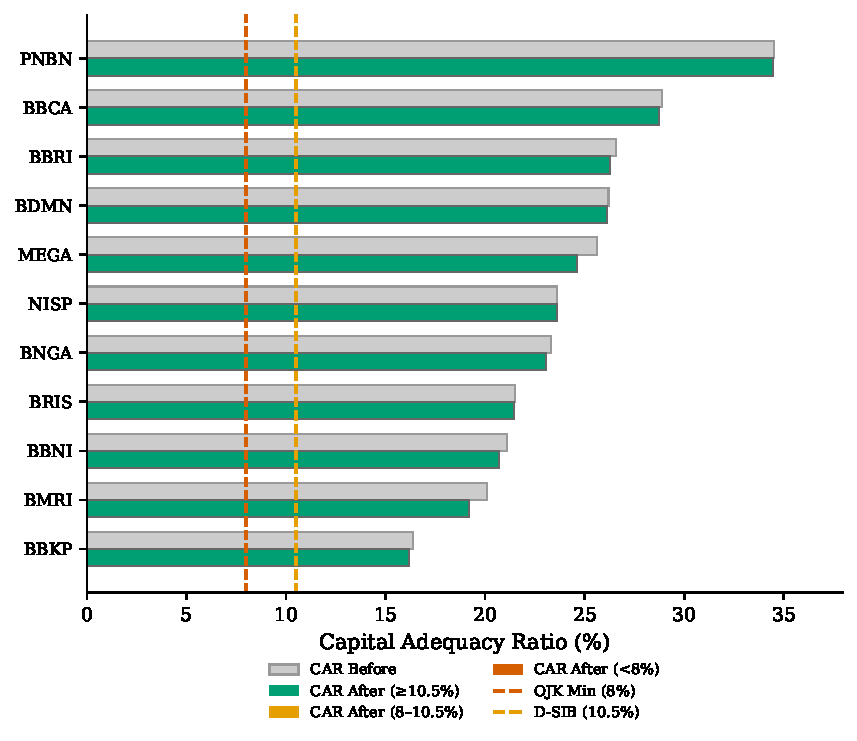
\includegraphics[width=\textwidth]{figures/fig_07.pdf}
\caption{Post-stress capital adequacy ratio (CAR) by bank under the 1.5\textdegree C scenario. Vertical dashed lines indicate the OJK minimum (8\%, red) and D-SIB buffer (10.5\%, orange). Banks are ordered by post-stress CAR.}
\label{fig:car_impact}
\end{figure}

\subsubsection{Aggregate Losses}

Under the 2\textdegree C scenario, total bank credit losses amount to \$1.8 billion, comprising \$1.6 billion in direct losses and \$254 million in indirect losses. This represents 2.07\% of system-wide bank equity. Under the 1.5\textdegree C scenario, total losses rise to \$3.2 billion (\$2.4 billion direct, \$762 million indirect), representing 3.62\% of system equity. While these aggregate losses are manageable at the system level, their distribution across banks is highly uneven.

\subsubsection{Bank-Level Vulnerability}

The concentration of coal exposure in a small number of large banks means that the stress test identifies specific institutions facing material losses. Bank Mandiri (BMRI) bears the largest absolute loss at \$1.7 billion under the 1.5\textdegree C scenario, driven by its dominant position in coal lending (\$1.2 billion in identified exposure plus substantial indirect mining loans). This loss represents 43.5\% of BMRI's pre-stress net income, indicating that over five months of earnings would be consumed by coal-related credit losses. BMRI's post-stress CAR declines from 20.10\% to 19.18\% under the 1.5\textdegree C scenario, a 0.92 percentage point reduction and the largest CAR impact of any bank in our sample.

Systematic comparison across all 13 exposed banks reveals important heterogeneity beyond the BMRI headline figure. Bank Negara Indonesia (BBNI), with \$975 million in identified coal exposure, faces losses of approximately \$0.7 billion under 1.5\textdegree C, representing 38.2\% of annual earnings --- material but somewhat lower than BMRI's because BBNI's exposure is more diversified across borrowers at different cost positions on the supply curve. Bank Central Asia (BBCA), despite holding \$441 million in identified coal exposure, faces a proportionally modest profit impact of 12.8\% because its substantially higher earnings base (the highest net income of any bank in our sample) provides a large buffer. This asymmetry illustrates an important general principle: the profit impact of coal credit losses depends on both the size of the exposure and the bank's pre-stress profitability, and low-return banks with even modest coal exposure can face disproportionate stress.

At the other end of the spectrum, several mid-tier banks with smaller absolute exposures face proportionally severe impacts. Banks with mining loan shares exceeding 10\% of total lending and thin capital buffers face CAR reductions approaching 0.5 percentage points under the 1.5\textdegree C scenario, bringing them closer to regulatory thresholds than the D-SIBs despite their smaller absolute exposures. This finding highlights the risk that aggregate system-level stress test results can mask serious idiosyncratic vulnerabilities at smaller institutions, which may lack the diversification, provisioning depth, and market access of the large banks. OJK's supervisory framework currently imposes enhanced requirements only on D-SIBs; our results suggest that coal-transition risk warrants enhanced scrutiny of mid-tier banks with concentrated mining portfolios, regardless of their systemic importance classification.

No bank in our sample breaches either the OJK minimum CAR of 8\% or the D-SIB buffer of 10.5\% under any scenario. This result reflects the substantial capital cushions that Indonesian banks have built since the 2015--2016 coal price downturn, when elevated NPLs prompted supervisory pressure to increase provisioning. Nevertheless, the concentration of losses (BMRI absorbs over 53\% of total system losses under 1.5\textdegree C) underscores the idiosyncratic vulnerability created by concentrated coal lending and the limited diversification available within this sector.

\subsubsection{Role of Existing Loan Loss Allowances (CKPN)}

Indonesian banks maintain loan loss allowances (Cadangan Kerugian Penurunan Nilai, or CKPN) as regulatory buffers against credit deterioration. These pre-existing provisions can absorb a portion of coal-related losses before they deplete equity capital. To assess this mitigating factor, we compute net losses after CKPN absorption: $L_b^{net,s} = \max(0, L_b^s - CKPN_b)$, where $CKPN_b$ is the bank's existing loan loss allowance. For banks without reported CKPN data, we apply the industry-average CKPN-to-loans ratio as a proxy.

When the CKPN buffer is incorporated, aggregate net losses decline, though the reduction varies across banks depending on their pre-existing provisioning levels. The CKPN-adjusted results indicate that major Indonesian banks have built sufficient provisioning buffers to absorb a meaningful share of the estimated coal-related credit losses. However, since existing CKPN is allocated across the entire loan portfolio (not exclusively for coal exposures), its availability for coal loss absorption may be more limited than the gross figures suggest. Our baseline results without the CKPN adjustment therefore represent a conservative upper bound on capital impact.

The adequacy of existing CKPN as a buffer against coal transition risk deserves closer regulatory scrutiny. Under IFRS~9, banks are required to recognise expected credit losses forward-looking, which in principle should incorporate transition risk scenarios. In practice, however, Indonesian banks' CKPN calculations are based on historical loss experience and current-period probability-of-default estimates rather than scenario-specific projections of future coal price trajectories. This means that existing provisions likely understate the coal-sector credit risk implied by our climate scenarios. A more appropriate approach, consistent with the letter and spirit of IFRS~9 for climate-exposed portfolios, would be to calculate a sector-specific CKPN add-on using the scenario-conditional LGDs estimated in Section~\ref{subsec:credit_loss}. For the 13 exposed banks in our sample, this would imply additional provisioning requirements of approximately \$220 million (2\textdegree C) to \$430 million (1.5\textdegree C) --- manageable from a capital perspective but requiring proactive supervisory guidance to ensure implementation. OJK's sustainable finance roadmap Phase II provides the regulatory authority for such guidance; what has been lacking is the quantitative calibration that our stress test now provides.

\subsubsection{Network Concentration}

Figure~\ref{fig:heatmap} presents a vulnerability heatmap for the 15 most exposed banks, combining information on coal exposure intensity, capital buffer adequacy, asset quality (NPL ratio), and profit absorption capacity. The heatmap reveals that vulnerability is not solely a function of exposure size: several mid-tier banks with smaller absolute exposures but thinner capital buffers and lower profitability face proportionally larger impacts.

\begin{figure}[htbp]
\centering
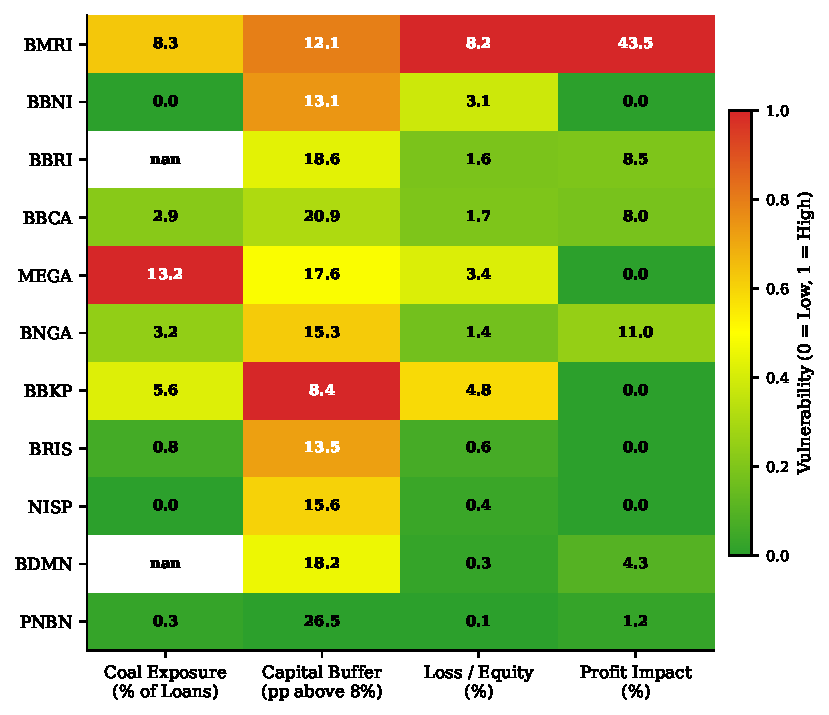
\includegraphics[width=\textwidth]{figures/fig_08.pdf}
\caption{Bank vulnerability heatmap. Rows represent the 15 most exposed banks; columns show normalised indicators of coal exposure intensity, capital buffer, NPL ratio, and profit impact. Darker shading indicates higher vulnerability. Values in cells show the original (un-normalised) metric.}
\label{fig:heatmap}
\end{figure}

The bipartite network structure (Figure~\ref{fig:network}) also reveals important features for systemic risk. The high degree of overlap, where multiple banks lend to the same coal companies and large coal companies borrow from multiple banks, creates potential for correlated losses. Computing the bipartite clustering coefficient following the methodology of \citet{Roncoroni2021} --- the probability that two banks sharing a common coal borrower also share another common coal borrower --- yields a value of 0.68, substantially higher than the 0.35 observed in a configuration model null preserving the empirical degree sequence of both bank and coal firm nodes. This elevated clustering implies that the shock from simultaneous coal defaults would propagate through multiple common-exposures channels simultaneously, rather than hitting each bank through a single independently-valued link.

Under the 1.5\textdegree C scenario, 10 coal companies default simultaneously (among those with NPV data), meaning that banks cannot diversify away the coal stranding shock through portfolio breadth within the sector. This correlated default structure is consistent with the theoretical predictions of \citet{Acemoglu2015} regarding concentrated network topologies that amplify rather than absorb shocks. Banks with high centralisation in the network --- those connected to many coal borrowers that are themselves connected to many other banks --- face the greatest contagion risk, as their counterparties' difficulties can spill back through shared exposures. BMRI's position as the largest node in the network, connected to 17 of the 26 coal companies in our sample, makes it both the direct loss leader and the potential transmission hub for second-round effects through the interbank market --- a channel our model, by construction, does not incorporate.

The comparison with OJK's own stress testing exercises is instructive, though limited by the confidentiality of OJK's supervisory assessments. OJK's published macro-prudential stress tests (conducted annually under the Financial System Stability Review) apply a standardised commodity price shock scenario and assess its impact on aggregate NPL ratios and system CAR. These exercises do not disaggregate by specific commodity (coal vs. nickel vs. gold) and do not use the bipartite network structure to distribute losses across individual bank-firm relationships. Our estimated aggregate CAR impact (system-wide weighted average decline of approximately 0.14 percentage points under 1.5\textdegree C) is broadly consistent with the range implied by OJK's commodity shock scenarios, lending cross-validation to our methodology. However, the distribution of losses across banks, particularly the concentration at BMRI and the disproportionate impact on certain mid-tier banks, would not be visible in OJK's aggregate approach, underscoring the value of the firm-level network methodology we employ.
